\documentclass{article}
\usepackage{graphicx}
\usepackage{amsmath}
\usepackage{float}


\title{\textbf{FYS4150/FYS1350 - Project 2}}
\author{Ingvild Bergsbak, Oliver Hebnes and Erlend Ousdal}
\date{October 1}




\begin{document}

\maketitle

\newpage

\section{Abstract}

Here we explore the use of Jacobi's rotation method when faced with eigenvalue problems. We develop an algorithm that will find the eigenvalues using Jacobi's method. The first problem introduce equations of a buckling beam. We find that our algorithms are extremely accurate when it comes to reproducing the eigenvalues found with numpys own eigenvalue-finder.  This allow for the use of theese algorithms in the second problem; the Schroedinger's equation for one and two electrons in a three dimensional harmonic oscillator well. Here we find that it is important to chose variables such as the number of integration points and the infamous $\rho_{max}$. For the one electron-system, the increase of N will grant better results when compared to analytical ones, but it also increase the cpu time. We found that if we need accuracy down to four leading digits while, the best choice is N=11 and $\rho_{max}$=4. When dealing with two electrons we find eigenvalues for the ground states of different frequencies $\omega_r$. We find that our choice of N and $\rho_{max}$ in this system grants stable results, and the eigenvalues increase as the frequency increase.  

\section{Introduction}

In this project we will be looking at eigenvalue problems



\section{Theoretical Models and Technicalities}

\subsection{Othogonal Transformation}
We have av orthogonal matrix so that
$$\mathbf{v}_j^T\mathbf{v}_i=\delta_{ij}$$
and othogonal transformation $\mathbf{w}$.\\
\vskip0.1cm
$\mathbf{w}_i=\mathbf{Uv}_i$\\
\vskip0.1cm
$\mathbf{w}_j^T\cdot \mathbf{w}_i=(\mathbf{Uv}_j)^T\cdot (\mathbf{Uv}_i)$
\vskip0.5cm
Calculating $\mathbf{Uv}_i$ and $(\mathbf{Uv}_j)^T$ separately.
\begin{equation*}
\mathbf{Uv}_i=\begin{bmatrix}
u_{11} & u_{12} & \cdots & u_{1n}\\
u_{21} & u_{22} & \cdots & u_{2n}\\
\vdots & \vdots & \ddots & \vdots\\
u_{n1} & u_{n2} & \cdots & u_{nn}\\
\end{bmatrix} \begin{bmatrix}
v_{i1} \\
v_{i2} \\
\vdots \\
v_{in} \\
\end{bmatrix}=\begin{bmatrix}
u_{11}v_{i1} + u_{12}v_{i2} + \cdots + u_{1n}v_{in}\\
u_{21}v_{i1} + u_{22}v_{i2} + \cdots + u_{2n}v_{in}\\
\vdots \\
u_{n1}v_{i1} +  u_{n2}v_{i2} + \cdots + u_{nn}v_{in}\\
\end{bmatrix}
\end{equation*}



\begin{equation*}
\begin{split}
(\mathbf{Uv}_j)^T&=\begin{bmatrix}
u_{11}v_{j1} + \cdots + u_{1n}v_{jn} &
u_{21}v_{j1} +  \cdots + u_{2n}v_{jn} &
\cdots &
u_{n1}v_{j1} + \cdots + u_{nn}v_{jn}\\
\end{bmatrix}\\
&=\begin{bmatrix}
v_{j1} &
v_{j2} &
\cdots &
v_{jn}
\end{bmatrix}\begin{bmatrix}
u_{11} & u_{21} & \cdots & u_{n1}\\
u_{12} & u_{22} & \cdots & u_{n2}\\
\vdots & \vdots & \ddots & \vdots\\
u_{1n} & u_{2n} & \cdots & u_{nn}\\
\end{bmatrix} \\
&=\mathbf{v}_j^T\mathbf{U}^T
\end{split}
\end{equation*}

$\mathbf{Uv}_i$ and $(\mathbf{Uv}_j)^T$ inserted back into the equation gives

\begin{equation*}
\begin{split}
\mathbf{w}_j^T\cdot \mathbf{w}_i&=(\mathbf{Uv}_j)^T\cdot (\mathbf{Uv}_i)\\
&=\mathbf{v}_j^T\mathbf{U}^T\mathbf{Uv}_i\\
&=\mathbf{v}_j^T\mathbf{I}\mathbf{v}_i\\
&=\mathbf{v}_j^T\mathbf{v}_i\\
&=\delta_{ij}
\end{split}
\end{equation*}

The orthogonal transformation preserves orthogonality and the dot product.

\subsection{Jacobi's Rotation Method}
For an eigenvalue problem
$$\mathbf{Ax}=\lambda\mathbf{x}$$
one can insert $\mathbf{B}=\mathbf{S^TAS}$ so that
$$\mathbf{B(S^Tx)}=\lambda(\mathbf{S^Tx})$$
which shows that $\mathbf{A}$ and $\mathbf{B}$ has the same eigenvalues, but different eigenvectors. This means that by finding the eigenvalues for $\mathbf{B}$ we also have the eigenvalues for $\mathbf{A}$.
\vskip0.5cm
Now we want to solve the eigenvalue problem using Jacobi's rotation method. The method uses orthogonal transformations to diagonalize the matrix by plane rotation around an angle $\theta$. The orthogonal transformation matrix is a $n\times n$ matrix on the form

\begin{equation*}
\mathbf{S}=\begin{bmatrix}
1 & 0 & & & \cdots & & & 0\\
0 & 1 & & & & & \\
 &  &\ddots & & & & &\\
\vdots &  & & \cos\theta & \cdots & \sin\theta & &\\
 & & &\vdots & \ddots & \vdots & &\\
 & & & -\sin\theta & \cdots & \cos\theta & & \\
 & & & & & & \ddots & \\
0 &  & & & \cdots  & & & 1\\
\end{bmatrix}
\end{equation*}

which has the property $\mathbf{S^T}=\mathbf{S^{-1}}$. The matrix has $1$ along the diagonal except $s_{kk}$ and $s_{ll}$ which is $\cos\theta$. Element $s_{kl}$ and $s_{lk}$ is $-\sin\theta$ and $\sin\theta$ respectively. All other elements are zero.

Performing the similarity transformation 
$$\mathbf{B}=\mathbf{S^TAS}$$
repeatedly will result in a diagonal matrix by choosing an appropriate value for $\theta$ for every transformation. We get $\mathbf{B}$ on the form

$$\mathbf{B}=\mathbf{S}^T_N...\mathbf{S}^T_1\mathbf{A}\mathbf{S}_1...\mathbf{S}_N$$

where $N$ is the number of transformations required to obtain a diagonal matrix.

One transformation has the objective of setting the highest non-diagonal element, $b_{kl}$, to zero which in the process changes the elements $b_{kk}$, $b_{ll}$, $b_{ik}$ and $b_{il}$ for all $i$ except $i=k,l$ the following way

\begin{equation*}
\begin{split}
b_{ik}&=a_{ik}\cos\theta-a_{il}\sin\theta\\
b_{il}&=a_{il}\cos\theta+a_{ik}\sin\theta\\
b_{kk}&=a_{kk}\cos^2\theta-2a_{kl}\cos\theta\sin\theta+a_{ll}\sin^2\theta\\
b_{ll}&=a_{ll}\cos^2\theta+2a_{kl}\cos\theta\sin\theta+a_{kk}\sin^2\theta\\
b_{kl}&=(a_{kk}-a_{ll})\cos\theta\sin\theta+a_{kl}(\cos^2\theta-\sin^2\theta)\\
\end{split}
\end{equation*}

$\theta$ is determined by demanding $b_{kl}=0$.

We perform the similarity transformations until all non-diagonal elements are zero, and we end up with a diagonal matrix. By definition the elements on the diagonal of a diagonal matrix, $\mathbf{D}$, are the eigenvalues of $\mathbf{D}$.
\vskip0.5cm
To find the analytical eigenvalues we used the numpy function linalg.eigvalsh.




\section{Results and Discussion}

\subsection{Similarity transformation}


For a given tolerance (we used eps$=10^{-15})$) we estimated the number of transformations found in figure \ref{simtrans}. If the dimension of a matrix increases, so will the number of similarity transformations.
But the scale is not linear, which means we should not neccesarily use this Jacobi's rotation algorithm for very big matrices because of the number of similarity transformations will increase with the dimensionality of the matrix.
If we time this with the number of flops in Jacobi's method (), it's easy to understand why we can draw this conclusion, and why it takes it very long time computing the eigenvalues, as seen in table \ref{timeusednumpy} and table \ref{timeusedjacobi}.


\begin{table}[H]
    \centering
    \begin{tabular}{|l|c|c|r|}
    \hline
     run & n=10 & n=20 & n=30\\
     \hline
      1  & 0.1043 s & 1.8843 s & 9.6493 s\\
      2  & 0.1004 s & 1.8887 s & 9.8702 s\\
      3  & 0.1053 s & 1.9206 s & 9.8153 s\\
      4  & 0.1027 s & 1.8263 s & 9.4729 s\\
      5  & 0.1002 s & 1.7854 s & 9.6888 s\\
      6  & 0.1053 s & 1.8869 s & 9.5218 s\\
      7  & 0.1014 s & 1.7886 s & 9.8120 s\\
      8  & 0.1052 s & 1.8935 s & 9.8537 s\\
      9  & 0.1094 s & 1.8524 s & 9.7283 s\\
      10 & 0.1002 s & 1.8545 s & 9.4581 s\\
      \hline
      Average & 0.10344 s & 1.85812  s & 9.68704 s\\
      \hline
    \end{tabular}
    \caption{Elapsed time for Jacobi's rotation method in Python with n equal the matrix dimension}
    \label{timeusedjacobi}
\end{table}

\begin{table}[H]
    \centering
    \begin{tabular}{|l|c|c|r|}
    \hline
     run & n=10 & n=20 & n=30 \\
     \hline
      1  & 0.000333 s & 0.000324 s & 0.000370 s\\
      2  & 0.000328 s & 0.000320 s & 0.000414 s\\
      3  & 0.000247 s & 0.000329 s & 0.000335 s\\
      4  & 0.000239 s & 0.000279 s & 0.000332 s\\
      5  & 0.000244 s & 0.000328 s & 0.000305 s\\
      6  & 0.000240 s & 0.000583 s & 0.000312 s\\
      7  & 0.000252 s & 0.000362 s & 0.000400 s\\
      8  & 0.000265 s & 0.000268 s & 0.000370 s\\
      9  & 0.000240 s & 0.000322 s & 0.000314 s\\
      10 & 0.000242 s & 0.000276 s & 0.000304 s\\
      \hline
      Average & 0.000263 s & 0.000339 s & 0.000346 s\\
      \hline
    \end{tabular}
    \caption{Elapsed time for Numpy's eigenvalue function in Python with n equal the matrix dimension.}
    \label{timeusednumpy}
\end{table}



%\begin{figure}
 % 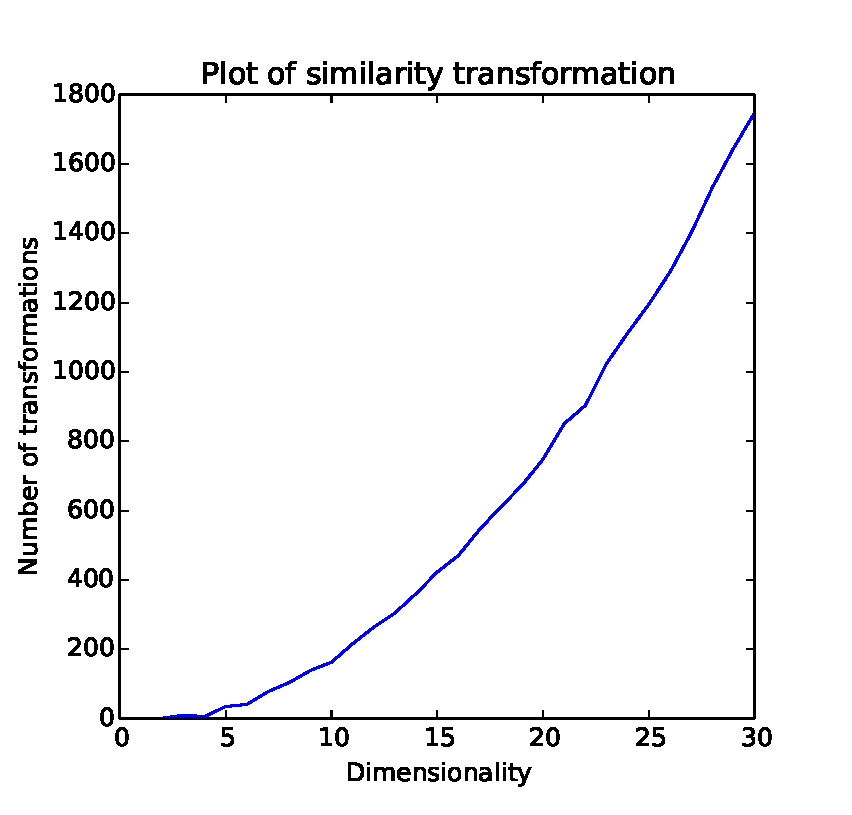
\includegraphics{simtransformations.eps}
  %\caption{Plot of the number of similarity transformations given by a tolerance of $10^{-15}$ without extending to quantum mechanics.}
 % \label{simtrans}
%\end{figure}





\subsection{Number of grid points and $\rho_{max}$ for the one electron system}

When modeling quantum dots in three dimension for one electron, the choice of the number of integration points N and $\rho_{max}$ is important to discuss. Chosing wrong values results in wrong eigenvalues when compared to the analytical results. From the project we know what the four first eigenvalues should be. In the project2.py program, different values for N and $\rho_{max}$ was tested through a loop.
It was quickly found that a $\rho_{max}=4$ gave the minimum difference from the analytical values, but the difference kept decreasing as N increased. Thus, we set the limitation such that the numerical eigenvalues should be equal to the analyitcal ones when using four leading digits. It was found that this happened when N=11, aswell as for bigger values of N. This means that when using four leading digits, we should use N=11 and $\rho_{max}=4$ to get the analytical results. Using theese values we got the result as presented in table \ref{tabelur1}

\begin{table}[H]
    \centering
    \begin{tabular}{|c|c|}
    \hline
     Nummerical eigenvalues & Analytical eigenvalues\\
     \hline
      2.965  &  3\\
      6.825  &  7\\
      10.61  &  11\\
      14.53  &  15\\
     \hline
    \end{tabular}
    \caption{Nummerical eigenvalues for N=11 and $\rho_{max}$=4}
    \label{tabelur1}
\end{table}

\subsection{Ground state eigenvalues for varying $\omega_r$}

When comparing the eigenvalues for the two-electron system, we use the same values for N and $\rho_{max}$ as before, N=11 and $\rho_{max}=4$. This gives us some interesting eigenvalues of the ground state of the system which can be found in table \ref{tabelur2}

\begin{table}[H]
    \centering
    \begin{tabular}{|l|c|}
    \hline
    $\rho_{max}$ & Nummerical eigenvalue \\
    \hline
    0.01 & 1.177  \\
    0.5  & 2.249  \\
    1.0 & 4.021  \\
    5.0 &  16.44  \\
     \hline
    \end{tabular}
    \caption{Ground state eigenvalues for N=11 and $\rho_{max}$=4 for different values of $\omega_r$}
    \label{tabelur2}
\end{table}

We see from the table that the eigenvalues increase as the frequency increase. This is as we have learned to expect from a one electron system, and it seems to be fitting for the two electron system aswell. Using Table 1 in \cite{M.Tant}, the energies also increase as the frequency increase.

\begin{thebibliography}{}
\bibitem{M.Tant}
M. Taut Two electrons in an external oscillator potential: Particular analytic solutions of a Coulomb correlation problem
\\\texttt{https://journals.aps.org/pra/abstract/10.1103/PhysRevA.48.3561}

\end{thebibliography}

\end{document}

